\mysection{Úvod}

V našom ročníkovom projekte, sme sa rozhodli zaoberať vizualizáciou distribuovaných algortimov
pomocou Java aplikácie, ktorá umožňuje jednoduché a rýchle pochopenie tématu, bez
študovania dlhých odborných textov.

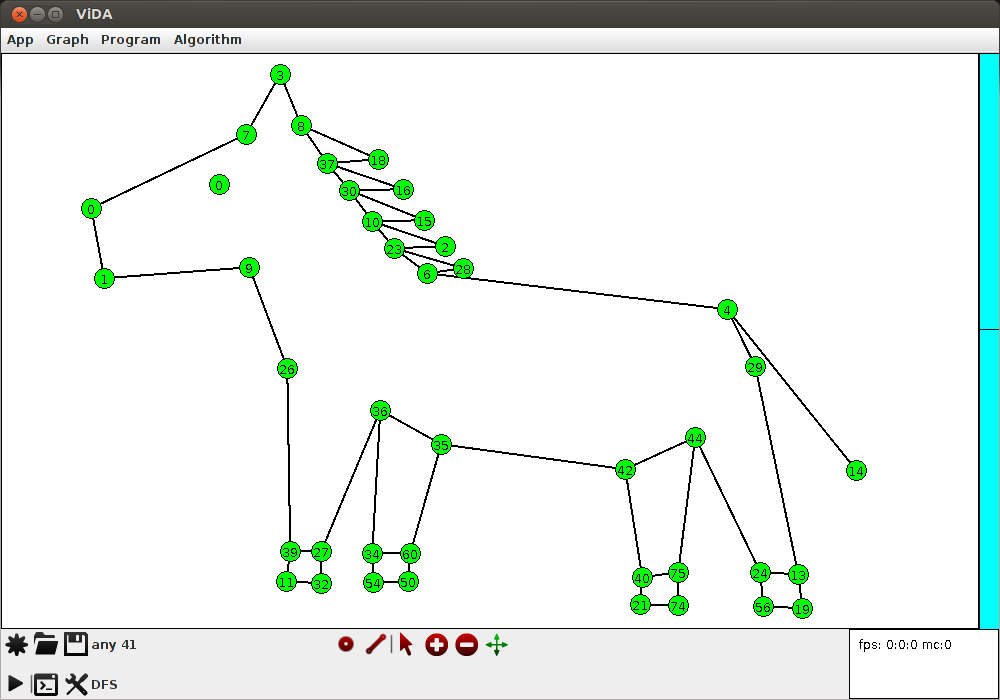
\includegraphics[width=\columnwidth]{konik}
%\caption{Vzhľad aplikácie po spustení}

\mysection{Distribuované algoritmy}

Vlastnosti modelu:
\begin{itemize}
    \item niekoľko počítačov zapojených do siete obojsmernými linkami
    \item majú jednoznačné id, komunikujú len správami
    \item správy sa nestrácajú, nemenia poradie, ale môže im to trvať ľubovoľne dlho -- asynchrónna
    komunikácia
\end{itemize}

Ciele:
\begin{itemize}
    \item poslať čo najmenej správ
    \item minimalizovať dobu behu algoritmu
\end{itemize}

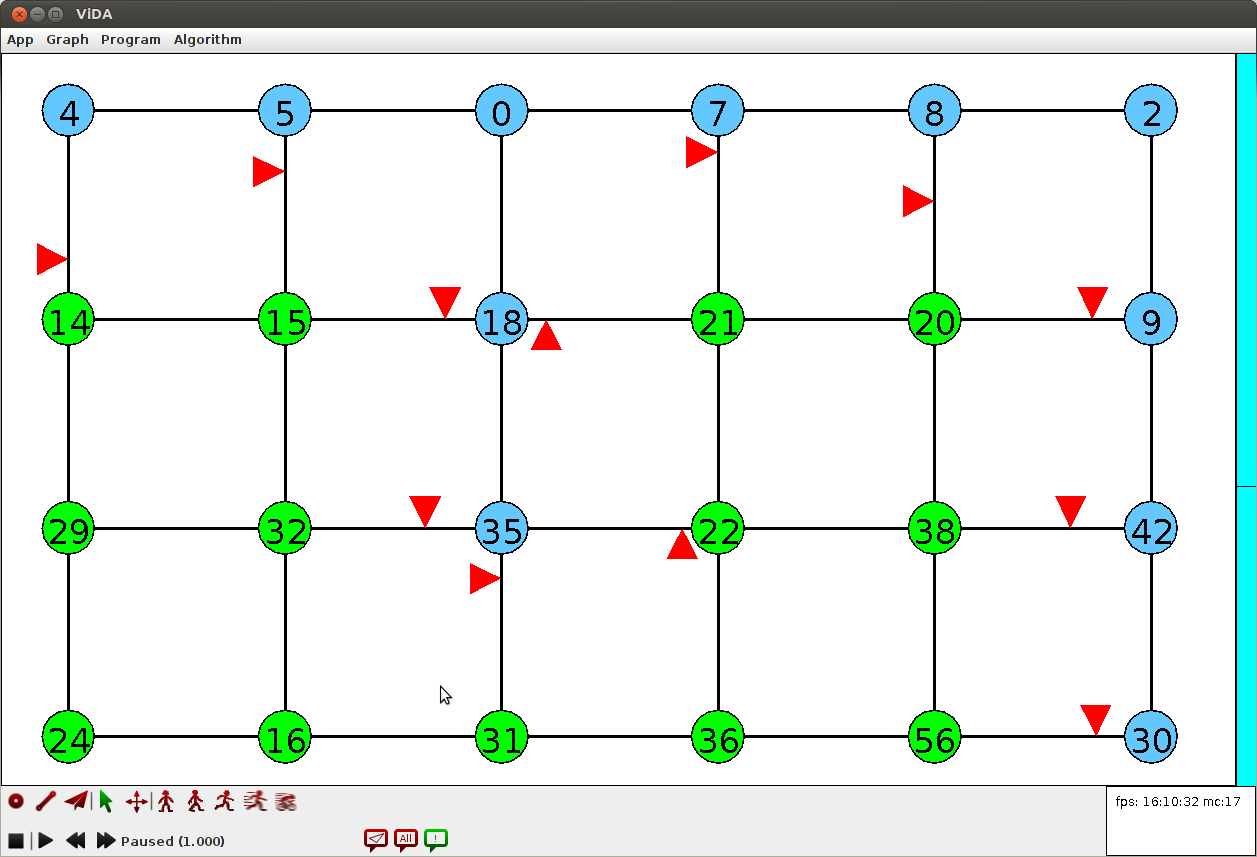
\includegraphics[width=\columnwidth]{asyn}
\caption{Asynchrónna komunikácia -- klebeta začala vľavo hore ( vrchol 4 ) a dostala sa na druhý
koniec mriežky ( vrchol 30 ) skôr, než do spodného suseda ( vrchol 14 ). Aj toto naša vizualizácia
dokáže spraviť. }
%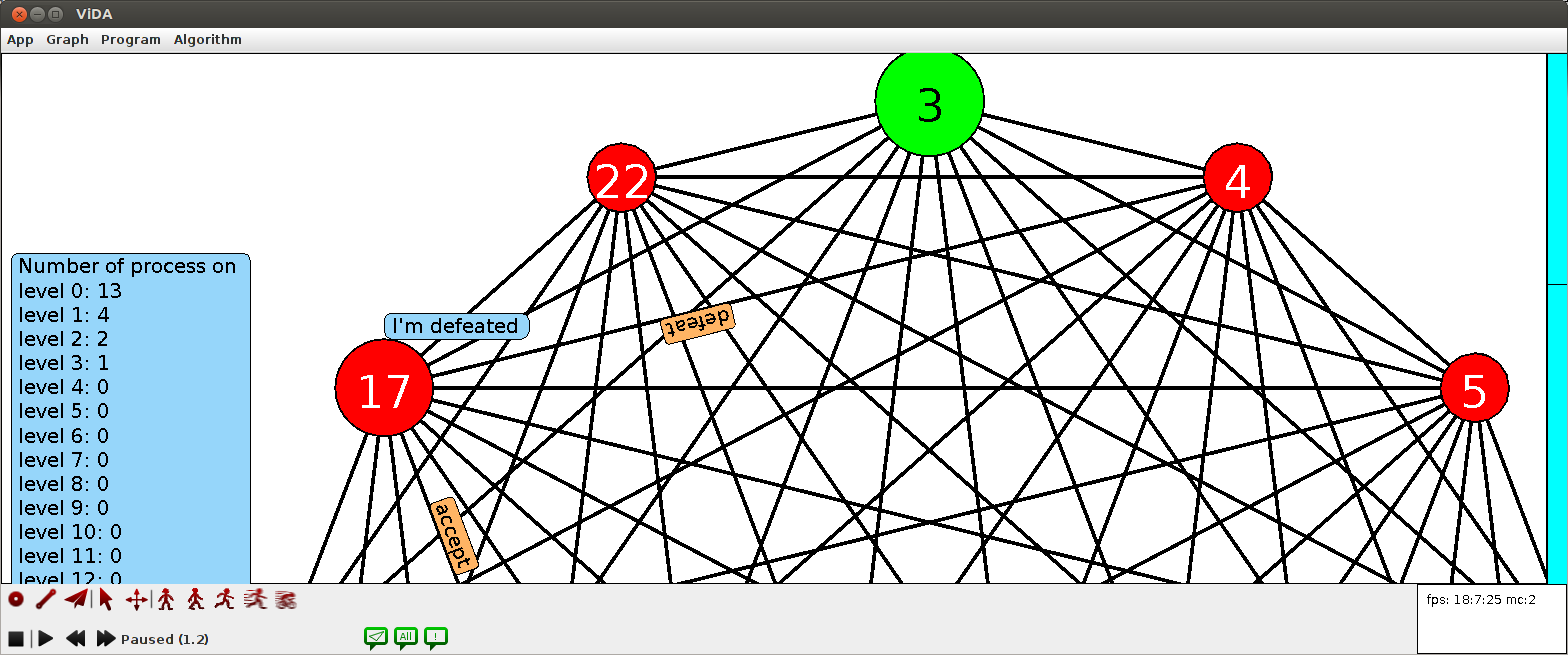
\includegraphics[width=\columnwidth]{le}

\mysection{Hlavné ciele}
\begin{itemize}

    \item vizualizácie ušité na mieru konkrétnym distribuovaným algoritmov
    \item interaktivita s používateľom
    \item prehľadnosť a jednoduchosť používania aplikácie
    \item schopnosť vizualizovať vlastné algoritmy

\end{itemize}

